\section{Efekt \textit{flanger}}

Ostatnim z~zaimplementowanych efektów był \textit{flanger}. Jest on wariacją poprzedniego efektu, w~której czasu opóźnienia jest wolnozmiennym sygnałem sinusoidalny o~niewielkiej amplitudzie. Jest ona najbardziej złożonym ze wszystkich zaimplementowanych bloków funkcjonalnych, jednak jego realizacja nie była wcale najtrudniejszym zadaniem. Wynikało to z~faktu, że komponenty potrzebnego do jego budowy - linia opóźniająca oraz generator funkcji sinus - zostały utworzone na wcześniejszych etapach projektu. Struktura zewnętrzna efektu została przedstawiona na Rys. \ref{flanger-structure}. Port \verb|depth| określa czynnik skalujący amplitudę sygnału opóźniającego. Jest interpretowana jako wartość z~zakresu $[0,1)$. Wejście \verb|strength| określa stosunek sygnału opóźnionego do~sygnału wejściowego w~wynikowej próbce. Wartości skrajne przekładają się na wyeliminowanie jednej ze składowych, natomiast wartość środkowa zakresu oznacza proporcję $1:1$. Ostatni z~parametrów - \verb|period| - kontroluje częstotliwość sygnału opóźnienia. Wyraża on (podobnie jak w~przypadku efektu tremolo) ilość cykli zegara systemowego przypadających na jedną próbkę LFO. Analogicznie do pozostałych modułów szerokości danych oraz poszczególnych parametrów mogą być ustalone za pomoca parametrów modułu (\textit{generic}).

\vspace{0.5cm}
\begin{figure}[ht]
    \centering
    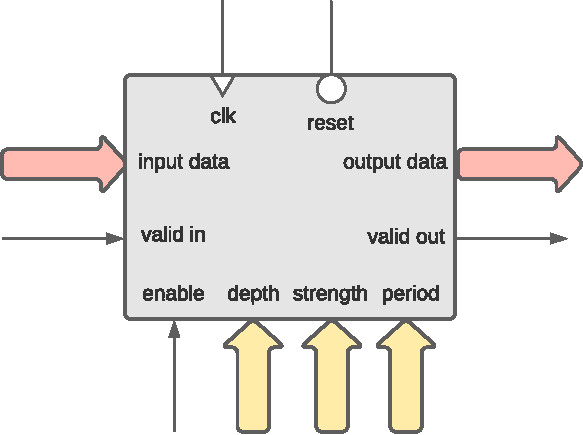
\includegraphics[scale=0.75]{img/diagrams/flanger.pdf}
    \captionsetup{format=plain,justification=centering}
    \caption{Struktura wyprowadzeń bloku \textit{flanger}}
    \label{flanger-structure}
\end{figure}
\vspace{0.5cm}

Zasada działania modułu jest syntezą działania efektów tremolo i~\textit{delay}. W~jego architekturze zaimplementowane zostały dwa procesy. Pierwszy z~nich odpowiada za generowanie kolejnych próbek LFO (jak w~przypadku tremolo). Z~kolei drugi inicjalizuje działanie linii opóźniającej oraz uaktualnia zawartość bufora wyjściowego (analogicznie do modułu \textit{delay}). Jeżeli wartość wejścia \verb|depth| była niezerowa w~momencie wykrycia stanu wysokiego na linii \verb|valid in|, to na wyjściu pojawi się wynik działania $x[t] \times (1 - S) + x[t-n] \times S$, gdzie $S$ jest wartością na porcie \verb|strength| interpretowaną jako liczba z~przedziału $[0,1)$. W~przeciwnym wypadku zapisana zostanie w~nim niezmodysikowana próbka wejściowa. Należy podkreślić, że w~przeciwieństwie do jednostki \textit{delay} wejście \verb|input data| bloku opóźniającego jest w~tym przypadku podłączone do \textbf{bufora danych wejściowych} efektu, a~nie danych wyjściowych. 

\vspace{1cm}
\begin{figure}[ht]
    \centering
    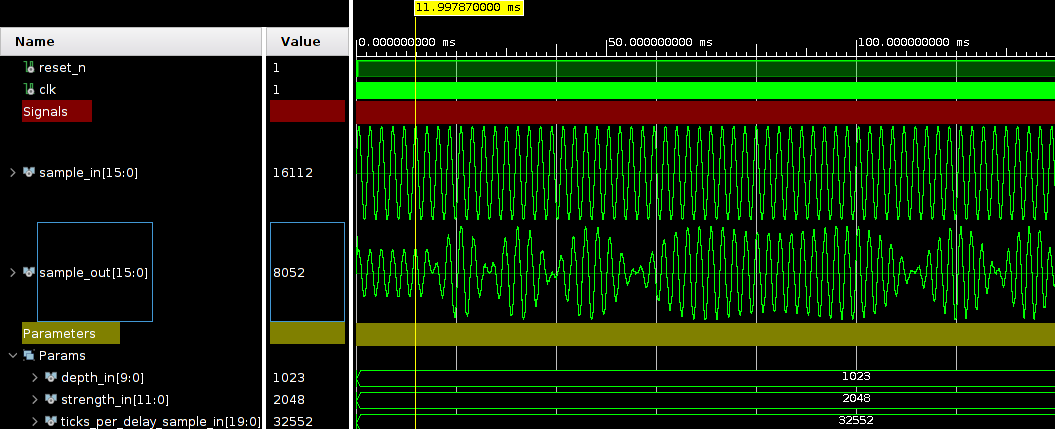
\includegraphics[width=\textwidth]{img/sim/flanger_sim.png}
    \captionsetup{format=plain,justification=centering}
    \caption{Fragment symulacji działania efektu \textit{flanger}}
    \label{sim-flanger}
\end{figure}
\vspace{0.5cm}

Na Rys. \ref{sim-flanger} przedstawiono fragment symulacji działania zaimplementowanego efektu dla częstotliwości oscylacji opóźnienia na poziomie $3$Hz i~amplitudy wartości $1024$ próbek oraz zrównoważonej proporcji sygnału opóźnionego i~wejściowego. Moment ustawienia linii \verb|enable| w~stan wysoki został oznaczony na rysunku źółtą flagą. Przebieg wartości wyjściowej modułu jest charakterystyczny dla działania efektu \textit{flanger}.

